
%
%  $Description: Author guidelines and sample document in LaTeX 2.09$
%
%  $Author: Gediminas Mazrimas $
%  $Date: 1995/09/15 15:20:59 $
%  $Revision: 1.4 $
%

\documentclass[times, 10pt,twocolumn]{article}
\usepackage{latex8}
\usepackage{times}

% Images includes
\usepackage{graphicx}
\usepackage{float}


%\documentstyle[times,art10,twocolumn,latex8]{article}

%-------------------------------------------------------------------------
% take the % away on next line to produce the final camera-ready version
\pagestyle{empty}

%-------------------------------------------------------------------------
\begin{document}

\title{Animating human model in OpenGL using data from Vicon system}

\author{Gediminas Mazrimas\\
Aalborg University Copenhagen\\ Computer Vision and Graphics\\g.mazrimas@gmail.com
\and
Algirdas Beinaravicius\\
Aalborg University Copenhagen\\ Computer Vision and Graphics\\algirdux@gmail.com
}

\maketitle
\thispagestyle{empty}

\begin{abstract}
   This paper explains how to animate 3D human model in OpenGL,
   using skeleton-driven deformation technique, similar to Linear Blend Skinning,
   that computes deformed weighted vertex position, which is calculated using quaternions.
   This helps to avoid some common animation problems, that occurs while dealing with
   various human body rigid parts transformations.
   The motion for this animation was captured using motion capture system
   and after processing it and converting to appropriate BVH format, was ready to use for
   animating 3D human model in lowest programming C++/OpenGL level.
   
   \textbf{Keywords:} Human animation, Vicon motion capture system, OpenGL, C++, Linear Blend Skinning
\end{abstract}



%-------------------------------------------------------------------------
\Section{Introduction}

Our animation focuses on the most common and partly simple human
body animation technique, that uses joint based structure to animate human model. Joint structure,
given their position and orientation, can be thought as being human body skeleton.
Animation of the skeleton, when talking about its complexity, is pretty simple,
as it includes only rigid body parts and requires rotations of bones at the joint position.
But when taking in account underlying layer of the skeleton, what we call skin, it becomes more
complicated. This is when linear blend skinning technique comes in use, associating joints to vertices and introducing weights them. Due to very fast computation speeds, this technique is the most popular
in animation production. On the other hand, using this simple shape blending technique
to deal with complex transformations, there are
various skin deformation problems. Typical ones are collapsing elbow, candy-wrapper joint
when the arm turns 180 degrees.
Also such a technique don't consider many other human body deformations, like stretching or bulging muscles.

%-------------------------------------------------------------------------
\SubSection{Previous works}

What we've read and what was written there. References.
[Linear blend skinning, for deformation problems, data formats, data format conversion problems (BVH) - this probably to be written somewhere else, maybe overview?]

%-------------------------------------------------------------------------
\SubSection{Overview}

We present a motion data driven technique of animating a human body model in OpenGL.
We have two main issues in this work, firstly getting motion data and using it 
correctly to animate skeleton and then solving the human model mesh deformation problems.
Using data captured by motion capture system and correctly defined joint structure,
we achieve realistic body movements for our model. Any motion data, that was captured
using same joint structure scheme as ours, can be used for animating that human body model.
\emph{Our human body model mesh was exported from Maya in T-pose or so called dress pose,
what is necessary to animate model correctly.}




TODO: Explain what are the problems,
kinematic chain,  what went wrong with stuff what we were doing,
what we could tell to other groups in order to continue with project,
emphasize that we use our joint model ant only take rotations.

%-------------------------------------------------------------------------
\Section{Linear blend skinning}

Linear blend skinning technique is widely used for interactive applications.
It goes by many different names, such as Skeleton Subspace Deformation or SSD or "smooth skinning" in Maya.

The linear blend skinning algorithm works by first placing a hierarchical
skeleton inside a static model mesh of a character in
some neutral pose (usually in the da Vinci posture or so called "dress pose").
Then, each vertex is assigned a set of influencing joints and a
blending weight for each influence. Computing the deformation in
some pose involves rigidly transforming each dress pose vertex by
all of its influencing joints. Then the blending weights are used to
combine these rigidly transformed positions.

The deformed vertex position, $ \overline{\textbf{v}} $ is
\begin{center}
$ \overline{\textbf{v}} = \displaystyle\sum_{i=1}^n\emph{w}_{i}M_{i}D_{i}^{-1}\textbf{v}_{d} $
\end{center}
where $w_{i}$ are the influence weights, $v_{d}$ is the dress-pose location of a
particular vertex \textbf{v}, $\emph{M}_{i}$ is the transformation matrix associated with
the $\emph{i}$th influence, and $D_{i}^{-1}$ is the inverse of the dress-pose matrix
associated with the $\emph{i}$th influence. Taken together, $D_{i}^{-1}\textbf{v}_{d}$ represents
the location of \textbf{v$_{d}$} in the local coordinate frame of the $\emph{i}$th influence.

\begin{figure}[H]
  \centering
  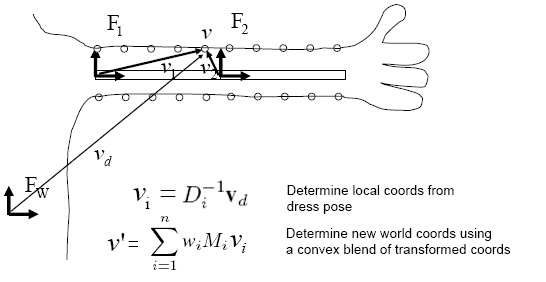
\includegraphics[width=93mm]{images/hand2.jpg}
\end{figure}

Linear blend skinning though has two primary failings.
First, the method is incapable of expressing complex deformations.
Artifacts such as the "candy-wrapper", collapse effect on wrists and
collapsing around bending joints as shown appear. They
occur because vertices are transformed by linearly interpolated matrices.
If the interpolated matrices are dissimilar as in a rotation of
nearly 180 degrees, the interpolated transformation is degenerate,
so the geometry must collapse.
Second, authoring linear blend skins is difficult and frustrating for users.

Despite its failings, this skinning algorithm is very fast and
widely supported by commercial applications so it remains popular
especially in games and virtual environments.

%-------------------------------------------------------------------------
\Section{Quaternions}

A quaternion is a mathematical object, consisting of 4 scalars. Quaternions were first discovered in 19th century by Irish mathematician Sir William Rowan Hamilton during his search for a way to represent points in space.  Soon after their introduction, quaternions appeared at most of universities as an advanced mathematics subject. Nowadays quaternions find their applications in signal processing, physics, bioinformatics, orbital mechanics as well as computer graphics.
	
In computer graphics Euler angles are known to have the disadvantage of being susceptible to "Gimbal lock" where attempts to rotate an object fail to appear as expected, due to the order in which the rotations are performed. Quaternions are a solution to this problem. Instead of rotating an object through a series of successive rotations, quaternions provide the ability to rotate an object through an arbitrary rotation axis and angle. Though the rotation is still performed by using matrix mathematics, instead of multiplying matrices together, quaternions, representing the axis of rotation, are multiplied together. The final resulting quaternion is then converted to the desired rotation matrix.

As mentioned earlier, a quaternion is four numbers, representing one real dimension and 3 imaginary dimensions. Each of it's imaginary dimensions has a unit value of square root of -1 (a complex number). In addition to that, imaginary dimensions are all perpendicular to each other and can be noted as i, j, k. So a quaternion can be represented as follows:
\begin{center}
q = \emph{a} + i$\ast$b + j$\ast$c + k$\ast$d
\end{center}
where \emph{a} is a real dimension representation and b,  c,  d are just scalars.

Since quaternions are mathematical objects, they have a certain algebra with all the addition, subtraction,  multiplication and division operations applied to them. In this section of the report we are going to consider just the quaternion multiplication operation, since this operation is necessary to represent a rotation. All other operations can be found in the references page of the report.

In order to perform a quaternion multiplication, a quaternion's imaginary dimension multiplication has to be described first:

\begin{description}
    \setlength{\itemsep}{0pt}

    \item \emph{i $\ast$ i = j $\ast$ j = k $\ast$ k = -1}
    \item \emph{i $\ast$ j = k}
    \item \emph{j $\ast$ i = -k}
    \item \emph{j $\ast$ k = i}
    \item \emph{k $\ast$ j = -i}
    \item \emph{k $\ast$ i =  j}
    \item \emph{i $\ast$ k = -j}
\end{description}

The multiplication of two quaternions is :

\begin{center}
(a + i$\ast$b + j$\ast$c + k$\ast$d) $\ast$ (e + i$\ast$f + j$\ast$g + k$\ast$h)

$\Updownarrow$

a $\ast$ e + i$\ast$a$\ast$f  + j$\ast$a$\ast$g + k$\ast$a$\ast$h + i$\ast$b$\ast$e - b$\ast$f  + k$\ast$b$\ast$g - j$\ast$ b$\ast$h + j$\ast$e$\ast$c - k$\ast$c$\ast$f - c$\ast$g + i$\ast$c$\ast$h + k$\ast$e$\ast$d + j$\ast$d$\ast$f - i$\ast$d$\ast$g - d$\ast$h

$\Updownarrow$

(a$\ast$e - b$\ast$f - c$\ast$g - d$\ast$h)  + i$\ast$(a$\ast$f + b$\ast$e + c$\ast$h - d$\ast$g) + j$\ast$(a$\ast$g - b$\ast$h + e$\ast$c + d$\ast$f) + k$\ast$(a$\ast$h + b$\ast$g - c$\ast$f + e$\ast$d)
\end{center}

The important thing to notice is that the multiplication of two quaternions is not commutative, so that
\begin{center}
q1 $\ast$ q2 $\neq$ q2 $\ast$ q1
\end{center}

As mentioned above, the multiplication operation,  provides us with the ability to rotate one quaternion by another quaternion. So the rotation of quaternion q1 by quaternion q2 would result in another quaternion q = q2 $\ast$ q1;

Since the representation of a quaternion is quite complex and hard to imagine, it can be interpreted in another way. The x, y, z components of a quaternion can be treated as a representation of rotation axis and a component - as a representation of rotation angle. The relation between actual values and their representations as quarternion's components can be described as:

\begin{itemize}
\item a = $cos(angle / 2)$
\item b =  $axis_x$ $\ast$ $sin(angle / 2)$
\item c = $axis_y$ $\ast$ $sin(angle / 2)$
\item d = $axis_z$ $\ast$ $sin(angle / 2)$
\end{itemize}
where $axis_x$, $axis_y$ and $axis_z$ is a normalized vector, representing the rotation axis.

In order to rotate a 3D point by a quaternion, a rotation matrix $R$ has to be produced:


\[ R = \left( \begin{tiny}\begin{array}{cccc}
a^{2}-b^{2}-c^{2}-d^{2} & 2 \ast b \ast c-2 \ast a \ast d & 2 \ast b \ast d+2 \ast a \ast c & 0 \\
2 \ast b \ast c+2 \ast a \ast d & a^{2}-b^{2}+c^{2}-d^{2} & 2 \ast c \ast d-2 \ast a \ast b & 0 \\
2 \ast b \ast d-2 \ast a \ast c & 2 \ast c \ast d-2 \ast a \ast b & a^{2}-b^{2}c^{2}+d^{2} & 0 \\
0 & 0 & 0 & 1
\end{array}\end{tiny} \right)\]






%-------------------------------------------------------------------------
\Section{Motion capture}

Motion capture (\emph{mocap}) is sampling and recording motion of humans, animals, and inanimate
objects as 3D data. The data can be used to study motion or to animate 3D computer models.
During the motion capture process not only the capturing stage using \emph{mocap} equipment
is very important, as equally important are the preparation and post processing processes.
The whole system must be well calibrated, adjusted and set up, furthermore, after capturing
data needs to be cleaned, edited, and applied to a 3D model.

During this project, for capturing motion data, we used Vicon Motion System,
combined with Vicon IQ 2.5 software running on our systems host pc.
Details on how we managed to capture and process motion data can be found on the appendix \textbf{\ref{Vicon appendix}}.


%-------------------------------------------------------------------------
\Section{Motion data}

There are various \emph{motion data} storing formats, that mostly depend on what kind of program they
are being used on. Our aim on this project, considering motion data, was to select
the most appropriate data format. After reviewing some examples, the decision was made,
that the best choice for our model animation would be using \emph{BVH} motion data format.
But because our motion capture is being done using Vicon IQ software,
that's not able to directly export data to BVH file format, at first we had to work with Vicons' C3D
and then convert it to BVH.

%-------------------------------------------------------------------------
\SubSection{Description of Vicon C3D format}

This section is meant to give just a brief introduction to the C3D file format, describing it in an abstract way. A reference to a detailed manual, describing the format, is given in the reference part of this document.

The C3D (Coordinate 3D) file format is a binary data file format originally developed for the AMASS photogrammetry software system, capable of storing 3D data as well as analog data together with all associated parameters for a single measurement trial. Since only the 3D data is of importance, we will not consider analog data in this document. The main advantage of C3D format over other motion capture data formats is that it is able to encapsulate the motion data as well as parameters, describing the  motion data, in a single file. Apart from that, C3D is freely licensed and well documented.

Being a binary file, the C3D file consists of a number of 512-byte blocks. Logically C3D format can be divided into 3 basic sections, each having one or more 512-byte blocks:
\begin{itemize}
\item Header section is the first section of a file. The main purpose of this section is holding a pointer to the start of parameters section. Other parts of this section, is of no particular importance, as usually it consists data, copied from parameters section.

\item The parameters section usually starts at block number 2, although this is not fixed and should not be assumed to be the case for every C3D file. This section contains information about the 3D data stored in the file. The section is extensible, meaning that user can define it's own parameters without  violating the format specification.

\item Data section containing the 3D point coordinates is usually located after the parameters section. This section simply contains sequential frames data. In the case of 3D points (the data is X, Y and Z coordinates).
\end{itemize}

%-------------------------------------------------------------------------
\SubSection{Description of Biovision BVH format}

The BVH format is an updated version of BioVision�s BVA data format, with the addition of a
hierarchical data structure representing the bones of the skeleton.
The BVH file is an ASCII file and consists of two parts.

First section (\emph{hierarchy}) is for storing hierarchy and initial pose of the skeleton,
basically joint-to-joint connections and offsets.
While as second section (\emph{motion}) describes the channel motion data for each frame,
that is describes the movement of individual joints.

The \emph{hierarchy} section starts with \emph{root} joint and contains the definition of a joint hierarchy within nested braces like source code written in the C programming language.
Each joint in a \emph{hierarchy} has an \emph{offset} field and a \emph{channels} field.
The \emph{offset} field stores initial \emph{offset} values for each joint with respect to its parent joint.
\emph{channels} field defines which �channels� of transformation (translation and/or rotation) exist for the joint in
the \emph{motion} data section of the file. The \emph{channels} field also defines the order of transformation. A
\emph{channel} is either x-, y-, or z-translation or local x-, y-, or z-rotation. All the segments are assumed
to be rigid and scaling is not available.
The \emph{end site} field is also available in order to determine body segment end.

In the \emph{motion} section the total number of frames in the animation and the frame
speed in frames-per-second is defined. Every next row then contains data values for all \emph{channels} which were specified in the \emph{hierarchy} section.
The listing order of \emph{motion} values in each row in is assumed to match their listed order from the \emph{hierarchy} section (top down).

There are few drawbacks of the BVH format. One is that it lacks a full definition of the initial pose. Another
drawback is that the format has only translational offsets of children segments from their parents. No
rotational offset can be defined. Moreover, the BVH format is often implemented differently in different
applications, that is, one BVH format that works well in one application may not be interpreted
in another. All the same the format is very flexible and it is relatively easy to edit BVH files.

\textbf{[Give more details later about exact structure of our model (like example)]}

%-------------------------------------------------------------------------
\SubSection{Processing motion data}

During the workflow of our project, the motion capture data, produced by the Vicon motion capturing system using Vicon IQ software, was encoded in C3D file format. This data in C3D file contains only the positions of the reflective markers at each frame. As it is not sufficient for us to correctly animate character, we have to do additional data processing.

\textbf{Only mention that conversion from C3D to BVH was made with 3rd part application?}

%We import C3D animation data file to MotionBuilder software. Then the whole data processing is similar to the one, that must be done after capturing data in post-processing stage, using Vicon IQ software. We assign the C3D motion data to so called actors and characters in MotionBuilder. Basically actor here is a mesh models, and character is skeleton with specified joint structure. As characters have their own skeleton, after assigning C3D data and using the inverse kinematics technique, we have whole body hierarchy and can export to BVH format, which contains the rotation and translation data of each joint for each frame.


\textbf{Forward Kinematics - The process of calculating the position and orientation of a specific part of an object based on the position and orientation of the root of the object as well as the position and orientation of the joints higher up in that part's kinematic chain.}


%\begin{figure}[H]
%  \centering
%  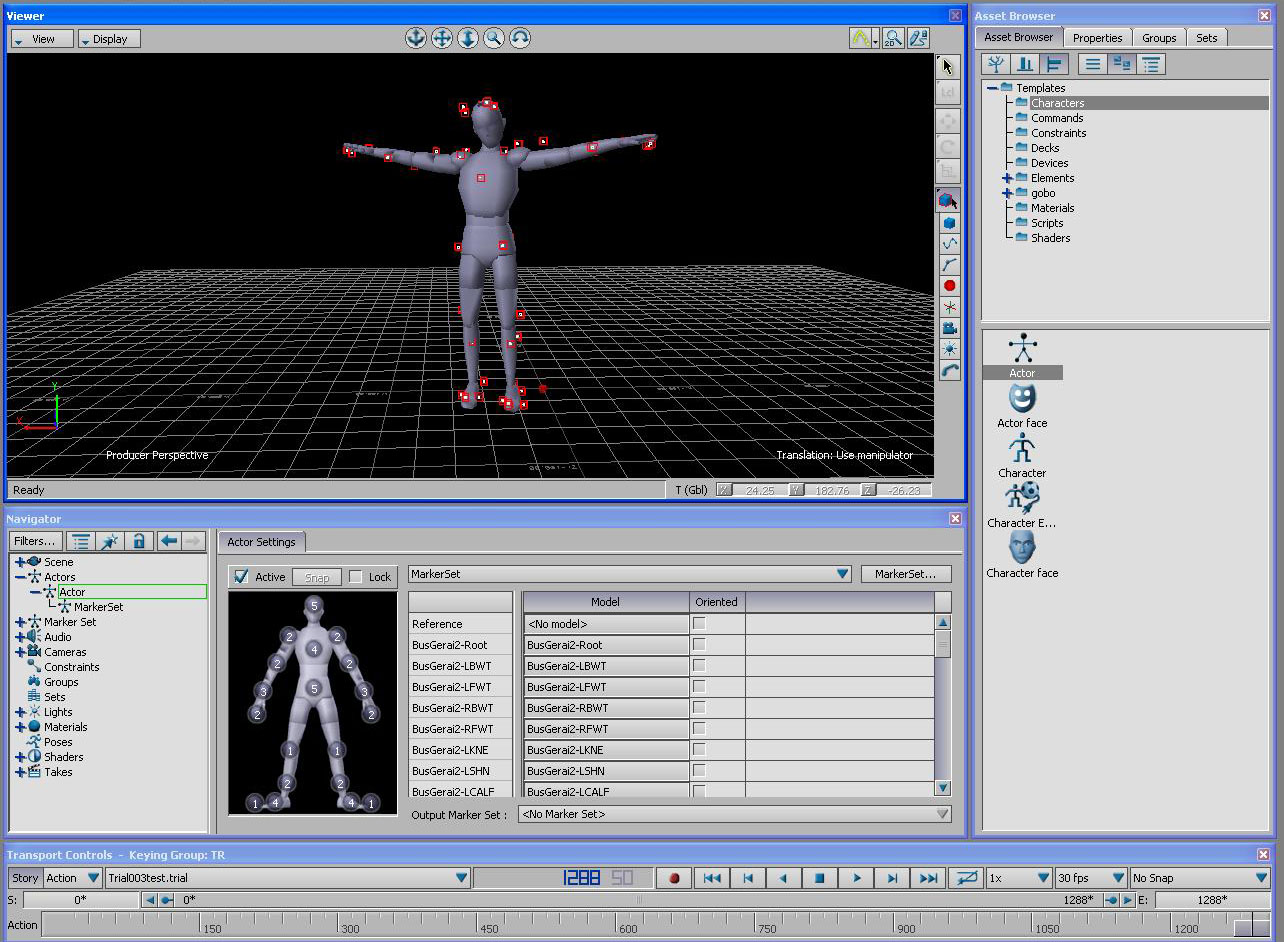
\includegraphics[width=85mm]{images/mb.jpg}
%\end{figure}

%-------------------------------------------------------------------------
\Section{Human body mesh model}

Human model mesh must be selected not only by it's looks and model details,
but also by its position. The model must be in such a position, that in
animating stage you could connect models body parts with your skeleton
and make it move. In this project simple human body mesh was selected with initial T-pose.

%-------------------------------------------------------------------------
\SubSection{Mesh model preparations}

Mesh model is a vital object in animation, looking from the users (viewers) side.
After using all the mathematical theories and different approaches, the final result
highly depends on the mesh being used.
For our project we decided to use whole human body mesh cut in different body parts,
with empty space between these rigid parts, that are later connected to one mesh.
The main issue using this kind of approach, is that you lose details of your body mesh,
so the better solution is using the whole uncut body.

\begin{figure}[H]
  \centering
  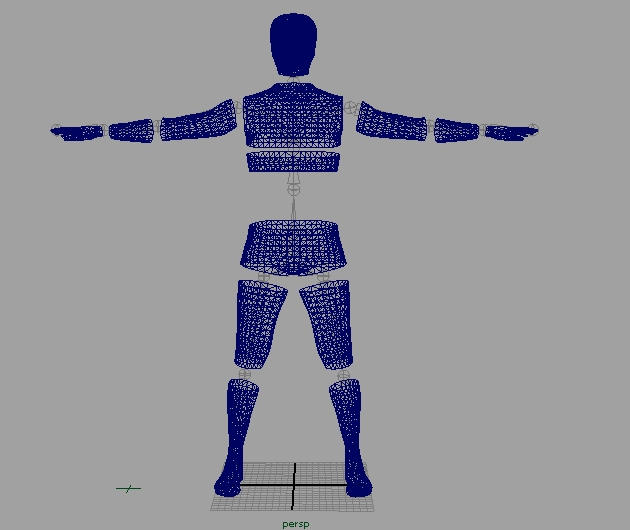
\includegraphics[width=85mm]{images/maya_cut.jpg}
\end{figure}

%-------------------------------------------------------------------------
\SubSection{Description of OBJ format}

OBJ is a geometry definition file format, first developed by Wavefront technologies. The file format is open and has been adopted by most of 3D graphics application vendors. It can be imported/exported from most of 3D modeling tools such as Autodesk's Maya, 3ds Max, Newtek's Lightwave, Blender, etc.  This section of the document provides a  thorough explanation of the most important parts of an object file, with more details provided in the reference page.

An object file can be stored in ASCII (using the ".obj" file extension) or in binary format (using the .MOD extension). The binary format is proprietary and undocumented, so only the ASCII format is described here.

The OBJ file format supports lines, polygons, and free-form curves and surfaces. Lines and polygons are described in terms of their points, while curves and surfaces are defined with control points and other information depending on the type of curve. Since, in our project, lines and polygons were sufficient to represent the model appropriately, only the parameters, concerning, these entities are described below.

The OBJ file is composed of lines of text, each of them starting with a token, which describes the type of the entity being  recorded in that line. Below are listed various tokens, which were of importance in our project:

\begin{itemize}
\item "\#" - a comment line. Lines, starting with "\#" token, are simply skipped by OBJ file readers. For example "\# this is a comment".
\item "g" - a group line. Lines, starting with "g" (group) token, determine the start of a group. "g" token is followed by the group name. For example $"g left_arm"$. In our project each group name corresponded to some body part, described by vertices, textures, normals and polygons.
\item "v" - a vertex line. Lines, starting with "v" (vertex) token, provide the information, concerning vertices. This token is followed by x, y and z coordinates of the vertex. For example "v -0.756447 0.702621 0.047024" is a vertex with coordinates (-0.756447, 0.702621, 0.047024).
\item "vt" - a texture line. Lines, starting with "vt" (vertex texture) token, are recorded with information, concerning textures. "vt" token is followed by x, y and z coordinates of the texture, although only the x and y coordinates are of importance (z coordinate is 0.0). For example "vt 0.487840 0.942165 0.000000".
\item "vn" - a vertex normal line. Lines, starting with "vn" (vertex normal) token, contain information, concerning the normal of a vertex. "vn" token is followed by x, y and z coordinates of the normal. For example "vn 0.149280 -0.186998 -0.240511".
\item "f" - a line, describing face. Lines, starting with "f" (face) token, provide the information, concerning polygons. "f" token is followed by a number of triplets, which is equal to the number of vertices, the polygon has. Each triplet is of a form "int/int/int", where the first "int" is a vertex position in the file, the second "int" is "texture" position in the file and the third "int" is a normal position in the file. For example "f 6/9/6 2/5/2 1/1/1" is a triangle polygon, with vertices 6, 2 and 1, textures 9, 5 and 1 and normals 6, 2 and 1.
\end{itemize}

The above described tokens were of importance in our project, but they are not the only ones that OBJ format allows. The OBJ format specification is much broader and covers such abilities as surface encoding, connectivity between free-form surfaces, rendering attributes. The OBJ specification can be found in the document's reference page.



%-------------------------------------------------------------------------
\Section{Animating human body}

Explain how we load human model, exported from Maya to .obj file.
How we create natural primary human pose, assign meshes to joints and so on.

\textbf{Having same joint structure in BVH file, we can animate any model, not having to worry about models height and so on, as using rotations we can animate differently sized model on our mesh/model.}

%-------------------------------------------------------------------------
\SubSection{Creating mesh model}
Loading rigid parts+Connecting rigid mesh parts

Loaded mesh from OBJ file must correspond with BVH file joint structure hierarchy. Cut mesh model should be connected in T-pose, otherwise program can't find closes vertices.

After we load OBJ file, we get every vertex of each mesh and its polygons connections.
Using this data we connect each of them to a mesh model.

How we load human body to OpenGL. How we import mesh from obj files.
Joint creation. Joint connection with meshes.

%-------------------------------------------------------------------------
\SubSection{Linear blend skinning relations}

How we adapted linear blend skinning to our animations.
Explain how our method using meshes assigned with joint rotations
is similar to linear blend skinning. How we automated all the things.


%-------------------------------------------------------------------------
\Section{Conclusion}
Conclusion

%-------------------------------------------------------------------------
\SubSection{Future work}
What could be implemented to improve this project?
Live streaming to our animating program (straight from cameras to animation in OpenGL);
other skin deformations

%-------------------------------------------------------------------------
\clearpage
\newpage

\appendix

\section{Details of using Vicon motion system}
\label{Vicon appendix}
\input vicon_appendix.tex

\clearpage
\newpage

\nocite{notseen}

%-------------------------------------------------------------------------
\nocite{ex1,ex5,ex2,ex3,ex4,ex6,ex7}
\bibliographystyle{latex8}
\bibliography{latex8}

\end{document}


